\section{Облачное хранилище лектория}\label{sec:cloud-storage}

%%%%%%%%%%%%%%%%%%%%%%%%%%%%%%%%%%%%%%%%%%%%%%%%%%%%%%%%%
\subsection{Основная информация}
%%%%%%%%%%%%%%%%%%%%%%%%%%%%%%%%%%%%%%%%%%%%%%%%%%%%%%%%%

Исходники с камер, шаблоны обложек, сцены и профили для OBS, таблицы с записью на предметы и для учёта лекций --- всё хранится на сервере в 2-ке. Доступ к серверу через веб из любого места осуществляется на платформе owncloud (скорость до 40 Мбит/с). На территории кампуса также есть возможность привязать сетевой диск по протоколу smb (cifs)\footnote{На установках в аудиториях диск обычно уже привязан с профиля \mitem{lectory-operator} и можно сразу загружать запись через проводник.} (скорость до 1 Гбит/c, \textbf{если это позволяет провайдер}). Больше технической информации можно найти в статье \href{https://wiki.stfpmi.ru/en/stfpmi/lectory/it}{IT-дела лектория}. Далее рассмотрим, как пользоваться каждым из этих способов.

%%%%%%%%%%%%%%%%%%%%%%%%%%%%%%%%%%%%%%%%%%%%%%%%%%%%%%%%%
\subsection{Owncloud}
%%%%%%%%%%%%%%%%%%%%%%%%%%%%%%%%%%%%%%%%%%%%%%%%%%%%%%%%%

Доступ через web: \href{https://drive.stfpmi.ru}{drive.stfpmi.ru}. После перехода по ссылке нужно нажать на поле \textit{\textbf{keycloak (stfpmi)}} и ввести учётные данные.

Для каждого пользователя заводится отдельная учётка. Чтобы её получить, нужно заполнить \href{https://forms.yandex.ru/u/64df964b02848f6809fb43af/}{форму}. В течение суток на указанную почту придёт пароль.

Иногда операторы не могут ждать в аудитории, пока лекция догрузится до конца на диск. В таком случае приходится оставлять компьютер докачиваться (лучше так не делать). Для таких сценариев была сделана общая учётка для операторов.

\hypertarget{lectory-operator-profile}{Данные от профиля оператора}:
\par\hspace{10pt} Логин: lectory-operator
\vspace{-5pt}
\par\hspace{10pt} Пароль: \_Учение-Свет\_

\vspace{5pt}

\textit{\textbf{Операторы}} загружают видео из аудиторий по пути:
\begin{itemize}
  \item <<Исходники для монтажа>> \ $\ra$ \ <<Raw>> \ $\ra$ \ <<OBS>> \ $\ra$ \ <<\,<год>.<месяц> - <название месяца>\,>> \ $\ra$ \ <<\,<дата>\,>> \ $\ra$ \ <<\,<название предмета и ФИО лектора>\,>>
\end{itemize}
Если промежуточных папок нет, нужно создать их самостоятельно, соблюдая формат. Пример пути: \textit{Исходники для монтажа/Raw/OBS/2024.02 - февраль/6 февраля/матан Лукашов}.

После того, как операторы загрузили исходники, записи обрабатываются на сервере и переносятся в другие папки. Поэтому \textit{\textbf{монтажёрам}} следует искать исходники по одному из следующих путей (в зависимости от того, на какую камеру велась запись):
\begin{itemize}
  \item <<Исходники для монтажа>> \ $\ra$ \ <<Processed>> \ $\ra$ \ <<OBS>> \ $\ra$ \ <<\,<год>.<месяц> - <название месяца>\,>> \ $\ra$ \ <<\,<дата>\,>> \ $\ra$ \ <<\,<название предмета и ФИО лектора>\,>> --- если занятие записывалось \textbf{на установку в аудитории}.
  \item <<Исходники для монтажа>> \ $\ra$ \ <<Processed>> \ $\ra$ \ <<Camera>> \ $\ra$ \ <<\,<месяц>\,>> \ $\ra$ \ <<\,<дата>\,>> \ $\ra$ \ <<\,<папка вида system\_...>\,>> \ $\ra$ \ <<\,source\_<время лекции>\,>> --- если занятие записывалось \textbf{на переносную камеру}.

        Переносных камер несколько, поэтому папок вида <<system\_...>> может быть несколько --- видео будет в какой-то из них. Рядом с записью будет лежать \textsf{.mp3} файл --- это запись звука на внутренний микрофон камеры. Она может пригодиться, если звук не записался на петличку.
\end{itemize}

%%%%%%%%%%%%%%%%%%%%%%%%%%%%%%%%%%%%%%%%%%%%%%%%%%%%%%%%%
\subsection{Сетевой диск (Windows)}
%%%%%%%%%%%%%%%%%%%%%%%%%%%%%%%%%%%%%%%%%%%%%%%%%%%%%%%%%

Переходите в проводник, пкм по \mitem{Этот компьютер} $\ra$ \mitem{подключить сетевой диск}.

\begin{center}
  \begin{minipage}[c]{\textwidth - \fboxaddlen}
    \centering
    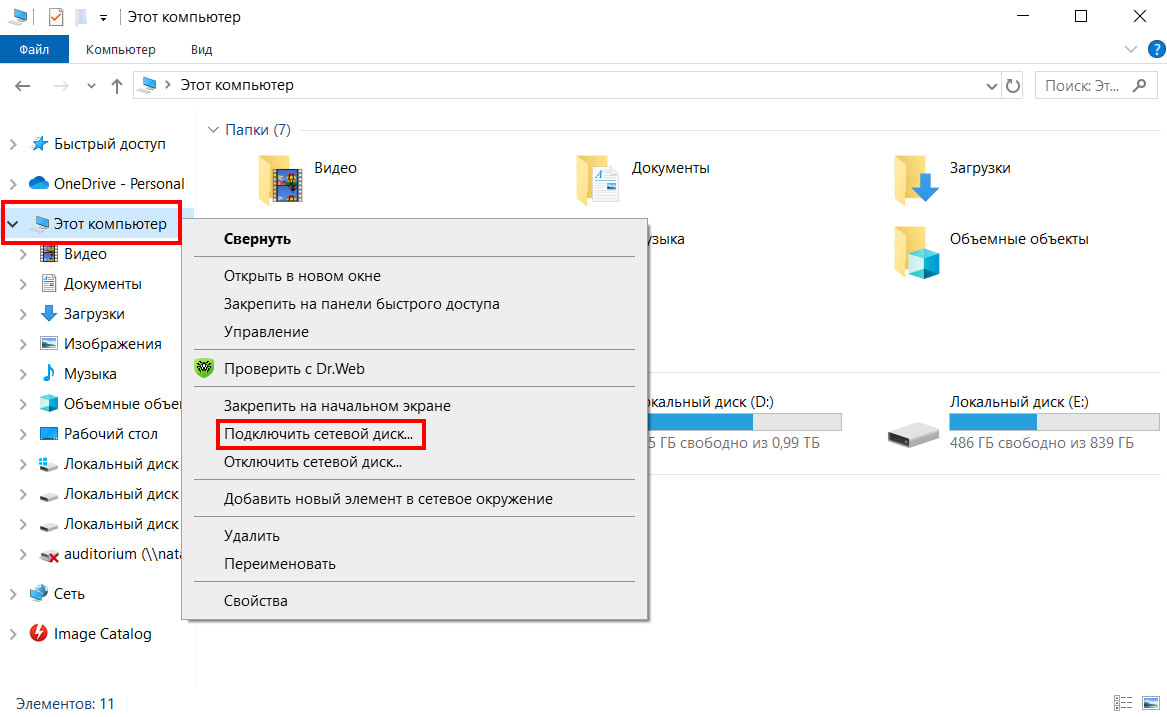
\includegraphics[width={\textwidth - \fboxaddlen},fbox]{Images/CloudStorage/windows/connect-network-drive.jpg}
  \end{minipage}
\end{center}

Выбираем любую доступную букву диска, помечаем оба флага и в поле \mitem{Папка} вводим адрес \mitem{\tbs\tbs drive.stfpmi.ru\tbs FpmiRaws}. Если диск не подключается, можно попробовать адрес \mitem{\tbs\tbs 93.175.2.3\tbs FpmiRaws}.

\begin{center}
  \begin{minipage}[c]{0.9\textwidth}
    \centering
    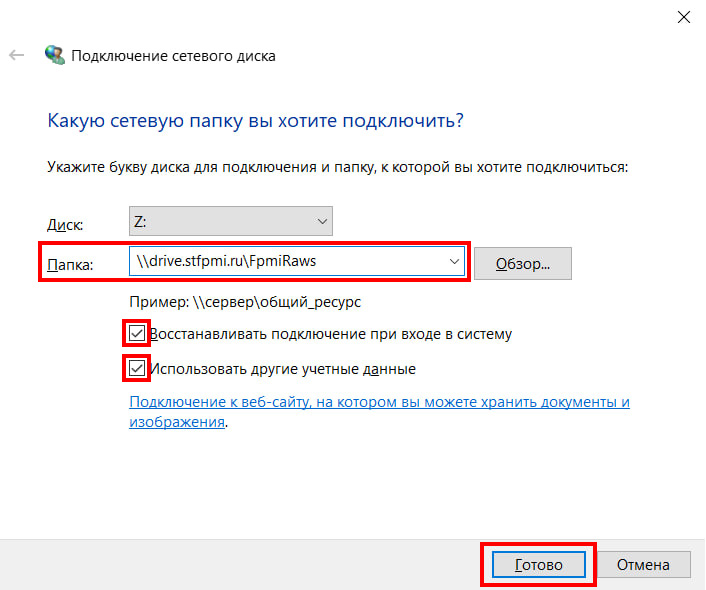
\includegraphics[width=0.9\textwidth,fbox]{Images/CloudStorage/windows/input-folder.jpg}
  \end{minipage}
\end{center}

Выбираем \mitem{Больше вариантов} \ $\ra$ \ \mitem{Использовать другую учётную запись} (если есть такое поле) и ставим флажок \mitem{Запомнить учётные данные}. Вводим данные от вашей учётки owncloud (либо от \hyperlink{lectory-operator-profile}{учётки оператора}, если вы подключаете диск на ПК в аудитории).

\begin{center}
  \begin{minipage}[c]{0.7\textwidth}
    \centering
    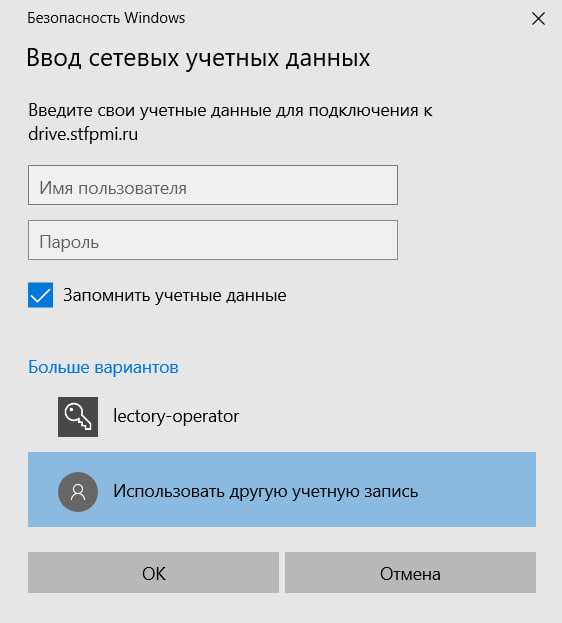
\includegraphics[width=0.7\textwidth,fbox]{Images/CloudStorage/windows/login.jpg}
  \end{minipage}
\end{center}

Исходники расположены по тем же путям, что и в owncloud, только без префиксной папки \mitem{Исходники для монтажа}.

%%%%%%%%%%%%%%%%%%%%%%%%%%%%%%%%%%%%%%%%%%%%%%%%%%%%%%%%%
\subsection{Сетевой диск (Linux)}
%%%%%%%%%%%%%%%%%%%%%%%%%%%%%%%%%%%%%%%%%%%%%%%%%%%%%%%%%

%%%%%%%%%%%%%%%%%%%%%%%%%%%%%%%%%%%%%%%%%%%%%%%%%%%%%%%%%
\subsubsection{Постоянная привязка (изменение /etc/fstab)}
%%%%%%%%%%%%%%%%%%%%%%%%%%%%%%%%%%%%%%%%%%%%%%%%%%%%%%%%%

Чтобы привязать диск, мы будем пользоваться командой \texttt{mount}. \href{https://losst.pro/montirovanie-diska-v-linux}{Тут} можно прочитать про саму команду и её параметры, а \href{https://ubuntuforums.org/showthread.php?t=288534}{тут} --- как настроить подключение по cifs (smb) протоколу, чтобы диск не удалялся после перезагрузки компьютера (раздел \mitem{Permanent mount}).

Краткая инструкция, как примаунтить диск с аккаунтом \mitem{lectory-operator}:
\begin{enumerate}
  \item Переключаемся в режим рута:
        \begin{tcolorbox}
          \texttt{sudo -iu root}
        \end{tcolorbox}

  \item Устанавливаем зависимости для работы с cifs:
        \begin{tcolorbox}
          \texttt{apt-get install -y keyutils cifs-utils}
        \end{tcolorbox}

  \item Создаём файл с логином/паролем:
        \begin{tcolorbox}
          \texttt{touch .smb\_operator\_credentials}
        \end{tcolorbox}

  \item Прописываем там данные от учётки. В случае учётки оператора:
        \begin{tcolorbox}
          \texttt{username=lectory-operator} \\
          \texttt{password=\_Учение-Свет\_}
        \end{tcolorbox}

  \item Меняем права файла, чтобы их мог читать только \texttt{root}:
        \begin{tcolorbox}
          \texttt{chmod 700 /root/.smb\_operator\_credentials}
        \end{tcolorbox}

  \item Теперь нужно внести изменения в файл \mitem{/etc/fstab}. \textbf{Этот файл используется системой для загрузки, поэтому редактировать его нужно с осторожностью}.
        \begin{itemize}
          \item Делаем резервную копию \mitem{fstab}:
                \begin{tcolorbox}
                  \texttt{sudo cp /etc/fstab /etc/fstab\_old}
                \end{tcolorbox}

          \item Открываем \mitem{/etc/fstab} и последней строкой добавляем:
                \begin{tcolorbox}
                  {
                    \small\texttt{//drive.stfpmi.ru/FpmiRaws \qquad /mnt/fpmi\_raws \qquad cifs \qquad credentials=/root/.smb\_operator\_credentials,uid=<username>,
                      gid=<username> 0 0}
                  }
                \end{tcolorbox}

                <<username>> нужно заменить на имя вашего пользователя linux. \textbf{В конце файла нужно обязательно оставить пустую строку}. Обратите внимание на табуляцию (лучше посмотреть на картинке). Файл будет выглядеть примерно так:

                \begin{center}
                  \begin{minipage}[c]{0.85\textwidth}
                    \centering
                    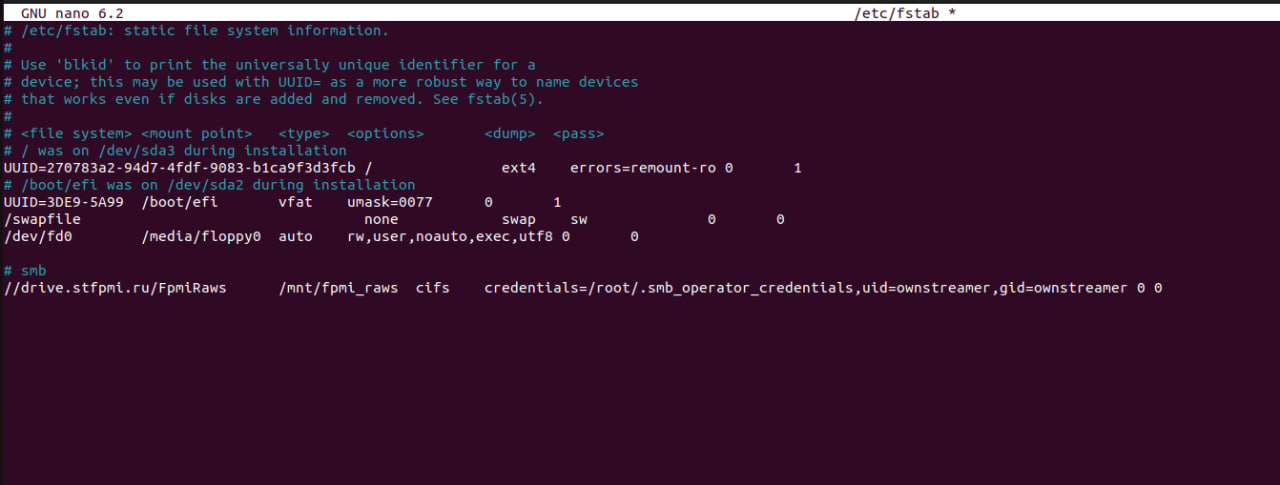
\includegraphics[width={0.9\textwidth},fbox]{Images/CloudStorage/ubuntu/fstab/fstab.jpg}
                  \end{minipage}
                \end{center}

          \item Выходим из файла, сохранив изменения.
        \end{itemize}

  \item Применяем изменения командой:
        \begin{tcolorbox}
          \texttt{mount -a}
        \end{tcolorbox}

  \item Проверяем, что диск подсоединился. Выходим из режима суперпользователя (команда \texttt{logout}) и проверяем, что существует папка <</mnt/fpmi\_raws>> --- в этой папке и будут лежать исходники. Если да, то вы успешно подсоединили диск и он будет автоматически цепляться при перезагрузке ПК.
\end{enumerate}

%%%%%%%%%%%%%%%%%%%%%%%%%%%%%%%%%%%%%%%%%%%%%%%%%%%%%%%%%
\subsubsection{Привязка на сессию (через nautilus)}
%%%%%%%%%%%%%%%%%%%%%%%%%%%%%%%%%%%%%%%%%%%%%%%%%%%%%%%%%

Если вы используете \mitem{nautilus} в качестве файлового менеджера, то подключить диск можно с помощью него. Недостаток такого подхода --- диск будет отсоединяться после перезагрузки ПК.

Нужно перейти на вкладку \mitem{Other Locations} и в поле \mitem{Connect to Server} ввести \mitem{smb://drive.stfpmi.ru/FpmiRaws}.

\begin{center}
  \begin{minipage}[c]{\textwidth - \fboxaddlen}
    \centering
    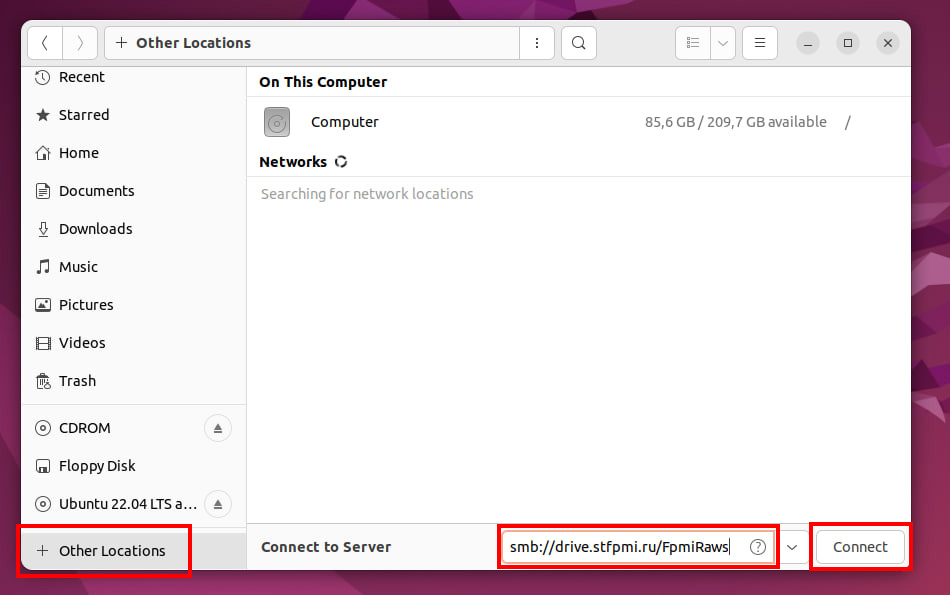
\includegraphics[width={\textwidth - \fboxaddlen},fbox]{Images/CloudStorage/ubuntu/nautilus/other-locations.jpg}
  \end{minipage}
\end{center}

После этого поставить флаг \mitem{Redistered User}, ввести ваш логин и пароль от owncloud. Флаг \mitem{Remember forever} позволит вам в будущем пропускать процесс ввода логина-пароля, но подключать диск после перезагрузки ПК всё равно придётся.

\begin{center}
  \begin{minipage}[c]{\textwidth - \fboxaddlen}
    \centering
    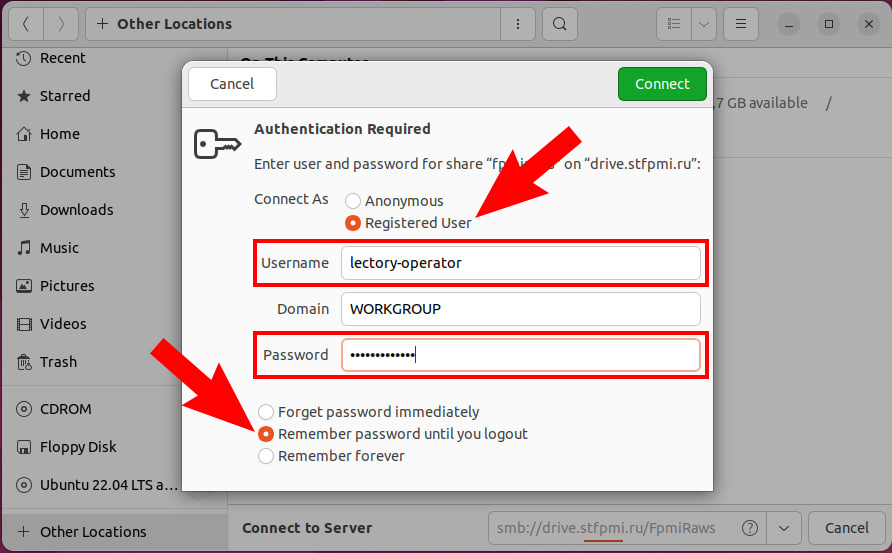
\includegraphics[width={\textwidth - \fboxaddlen},fbox]{Images/CloudStorage/ubuntu/nautilus/auth.jpg}
  \end{minipage}
\end{center}

После успешного подключения диск должен появиться в группе \mitem{Networks} как на фото, а также в во вкладке \mitem{Other Locations}.

\begin{center}
  \begin{minipage}[c]{\textwidth - \fboxaddlen}
    \centering
    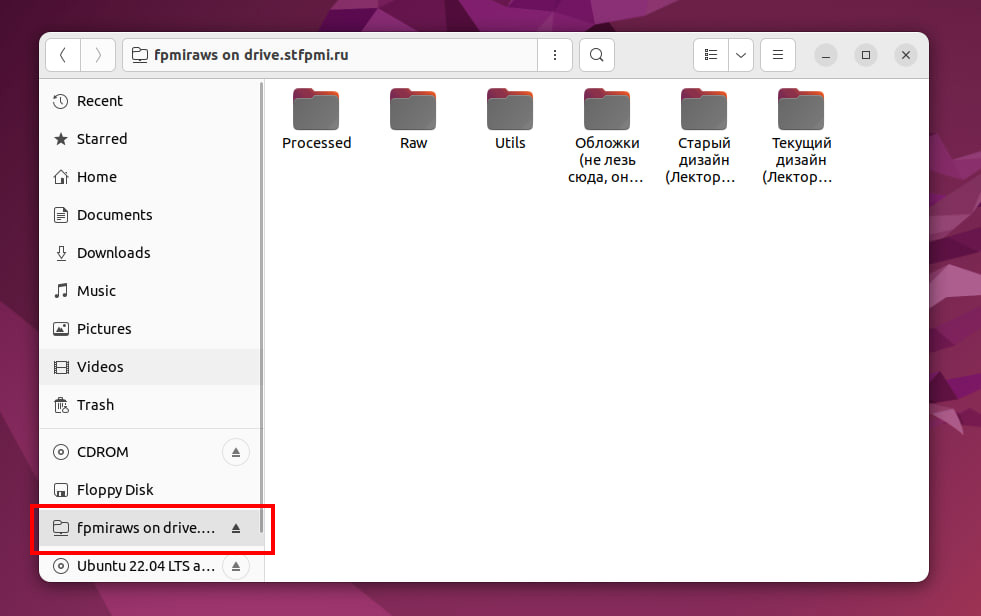
\includegraphics[width={\textwidth - \fboxaddlen},fbox]{Images/CloudStorage/ubuntu/nautilus/folder-in-tray.jpg}
  \end{minipage}
\end{center}
